
\section{Equivalent Linear Method}

The most common manifestations of inelastic soil behavior involve the reduction in shear wave velocity and the increase in soil damping with increasing load. The technical implementation for one dimensional domain is presented in numerous sources \citep[e.g.,][]{Kramer1996geotechnical}. In three dimensional domain we consider the following steps: First we run the simulation and extract the strain level of each element. Then we compute the effective strain for each time step. The computation of effective strain will be discussed later. We keep the maximum effective strain through the simulation time. Based on effective strain we update the material damping and shear modulus. We repeat the iteration up to 10 times. For a time being we do not related the simulation to the convergence of strain level, however, our results represent a very good agreement (convergence) after 3-5 iteration. The convergence factor may vary with increasing geological complexity of the domain and source slip function and frequency. Fig.~\ref{fig:equivalent_linear_flowchart} presents the equivalent linear work flow. 

\begin{figure}[H]
    \centering
    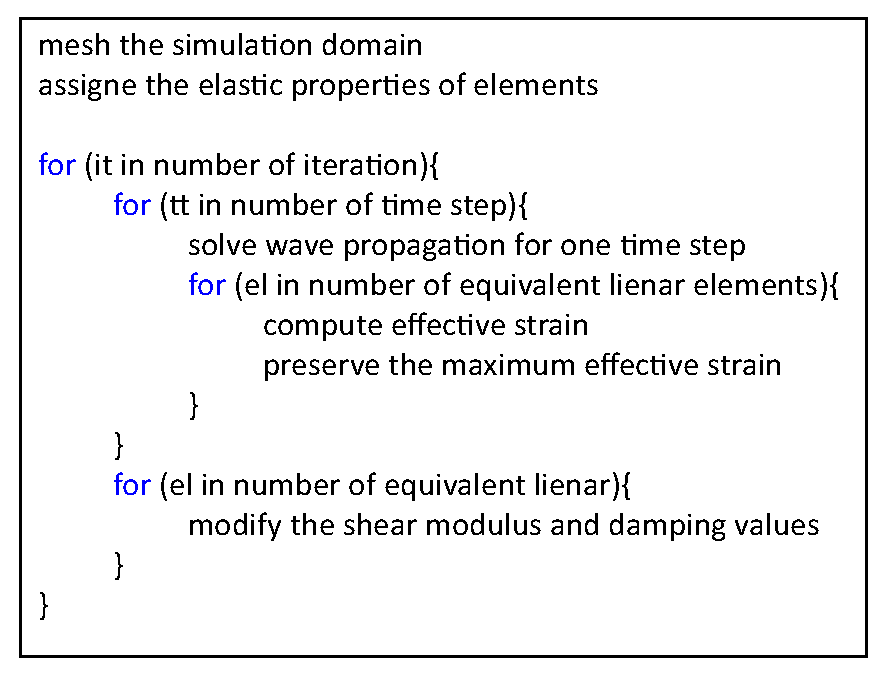
\includegraphics[width=300px]{figures/pdf/equivalent_linear_flowchart.pdf}
    \caption{Equivalent linear flowchart}
    \label{fig:equivalent_linear_flowchart}
\end{figure}


\subsection{Effective Strain}

Determination of effective strain is the most important part of application of equivalent linear method in 3D ground motion simulation. In 1D simulations the effective strain is related to the shear strain of the elements (or soil layer in case of frequency domain analysis) with some modification factor. The maximum strain level of typical earthquake motion can happen at a few spikes in the record. Therefore, the maximum strain level should not be dominant value in determining the effective strain. In literature effective shear strain is defined as 50 ~ 70\% of the maximum shear strain. This value mostly is considered as 65\% \citep{Kramer1996geotechnical}.  \citet{Idriss1992} proposed to use 

\begin{equation}
R_{\gamma} = \frac{M-1}{10}
\end{equation}

 relation for determining the effective shear strain. Where M is the magnitude of earthquake. The fact that effective shear strain is related to the incoming force is also addressed in \citet{Lysmer1975}. They proposed to consider a control motion (which could be a station at rock outcrop) and define and extra value for effective strain as 
 
 \begin{equation}
c = \frac{max|\ddot{y}(t)|}{RMS(\ddot{y}(t))}
\end{equation}

where $\ddot{y}(t)$ is the control motion and RMS is root mean square function. $c$ is the additional scaling factor for effective strain to be used in 

\begin{equation}
\gamma_{eff}=0.65*c*RMS(\gamma_{max})
\end{equation}

 \citet{Lysmer1975} computed the $\gamma_{max}$ using
 
 \begin{equation}
 \gamma_{max}^{2} = (\epsilon_{x}-\epsilon{y})^2 + \gamma_{xy}^{2}
 \end{equation}
 
where $x$ and $y$ present horizontal and vertical components, respectively.  The effective strain level proposed by \citet{Lysmer1975} considers only two components. However, in fully 3D simulation all three components should be considered. In this study we consider the following equation for determination of effective strain.

 \begin{equation}
 \gamma_{max} = G(A \gamma_{xy}^{2} + B\gamma_{xz}^{2} + C\gamma_{yz}^{2} + D(\epsilon_{x}-\epsilon_{y})^2 +E(\epsilon_{x}-\epsilon_{z})^2+F(\epsilon_{y}-\epsilon_{z})^2)^H
 \end{equation}
 
 where $\gamma$ and $\epsilon$ show shear and normal strains, respectively. Calibration of parameters to match the results with observation is common practice in application of equivalent linear method.  \citet{Assimaki2006attenuation} vary the soil profiles from the measured values to improve the fit. 

 
